\section{Set-up of the scene}
The modeling of the scene has been done with the 3D-graphics software \textit{blender}. Figure \ref{fig:blender} shows a screen-shot with the model used for the cloth simulation. Once, the wire-frame and the texturing is done, the model is exported as wavefront object. The result is a \textit{.obj}-file and a \textit{.mat}-file. In a post-processing step with the \textit{blender2oGL} \footnote{The \textit{blender2oGL} tool is available from our project repository on GitHub: \url{https://github.com/3eee3/ez-dc-ga}.} tool, also developed during the project, the \textit{.obj}-file is translated to a set of C-source and header files, ready to include into the project. Thus, almost any scene setting is easily included into the cloth simulation program, as long as the target computer can handle the processing effort\footnote{The algorithms to compute the physics simulation and the collision detection are quite CPU-time expensive. Besides that, the computation is forced onto one single core, such that only small scenes will run smooth and seamless.}.
\begin{figure}[h]
	\centering
	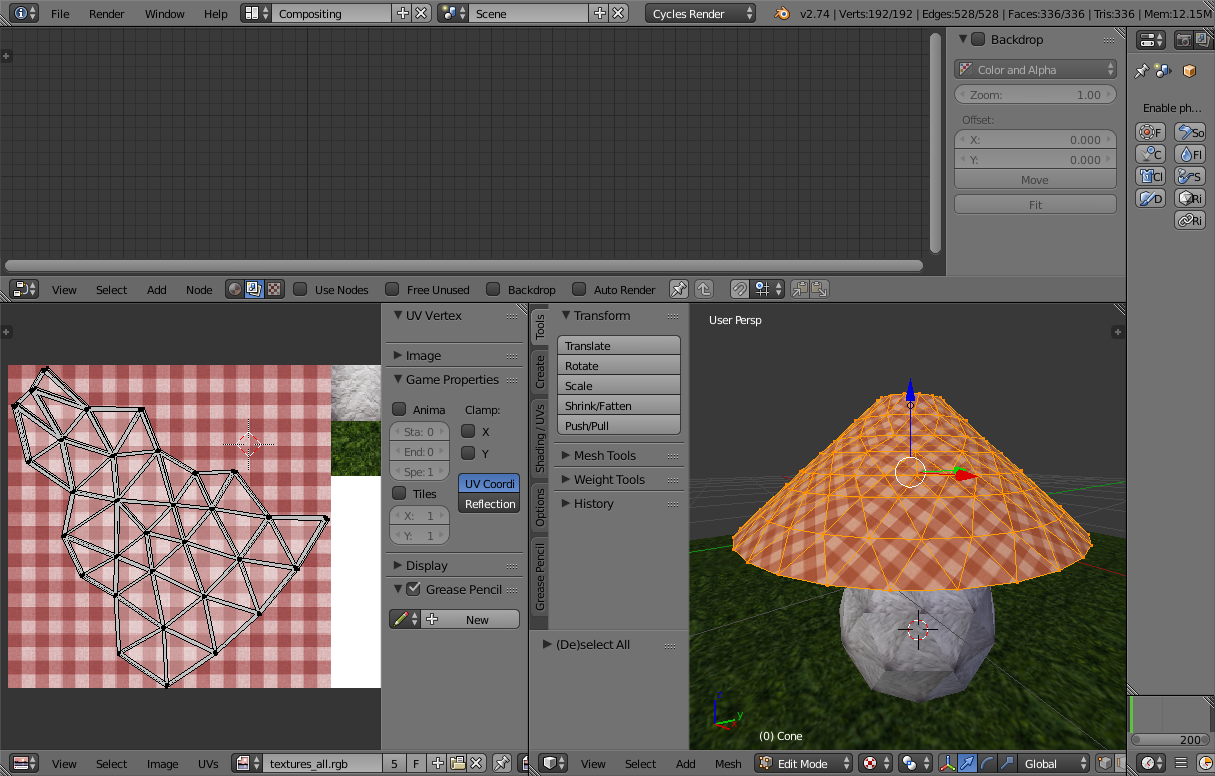
\includegraphics[width=\textwidth]{skirt_sphere_blend}
	\caption{Blender is used to set up a model. Subsequently, the model is exported as wavefront object file and converted to C-files with the \textit{blender2oGL} tool.}
	\label{fig:blender}
\end{figure}

The initial setting shows a skirt above a sphere. The sphere is hovering above the ground. As shown in figure \ref{fig:scene_wrap}, the skirt falls down, on top of the sphere and wraps around it. After the collision with the surface of the sphere, the cloth slips off, driven by the gravity, applied to the not exactly centered cloth. The penalty force of the collision detection algorithm has also an effect which drives the skirt off the sphere. Finally, the skirt falls down to the floor, where it collides with many wrinkles.\par
We decided to implement different scenes for debugging reasons\footnote{During the implementations happened some obstacles which led to non-running code. Because of that, we created a reduced version of the \textit{skirt} program without the connection to the \textit{blender} generated model. It contains a hard-coded grid of masses and springs with two corners fixed on top. It is also available on our project repository.}. So, a second scene with two dice is available by uncommenting the line
\begin{verbatim}
#define _DEBUG_OGL_MODEL
\end{verbatim}
in the file \textit{model\_mapping.cpp}.

\begin{figure}[h]
	\centering
	\begin{subfigure}{0.48\textwidth}
		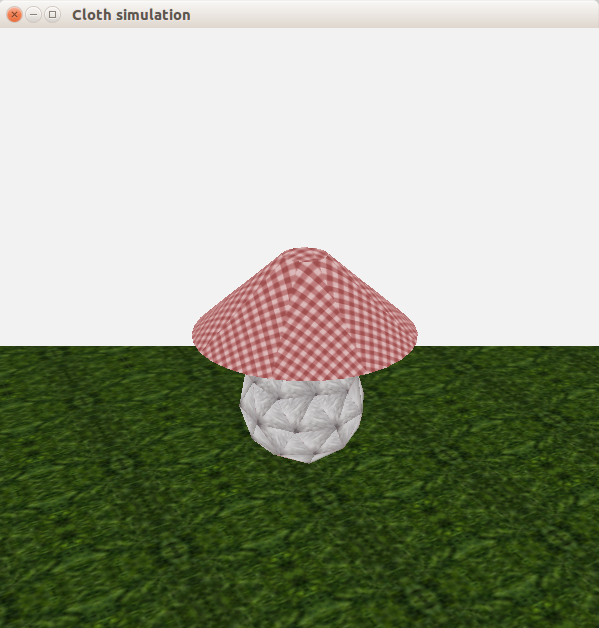
\includegraphics[width=\textwidth]{cloth_sim_initial_scene}
		\subcaption{Initial scene.}
		\label{fig:scene_init}
	\end{subfigure}
	\\
	\begin{subfigure}{0.48\textwidth}
		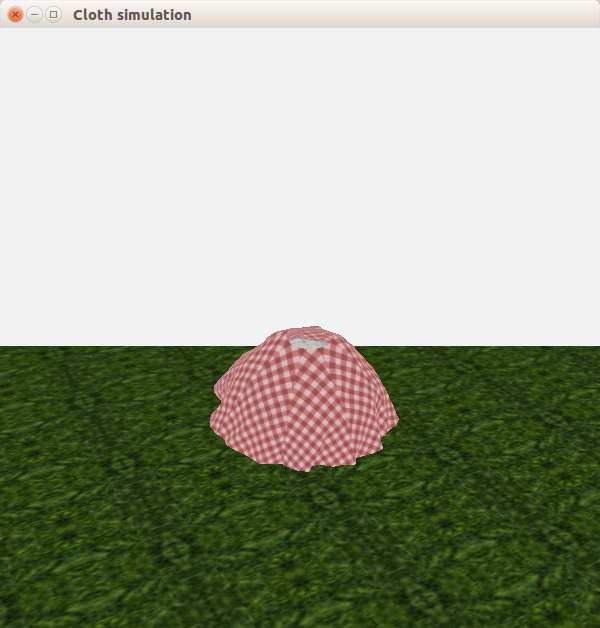
\includegraphics[width=\textwidth]{cloth_sim_wrapped_sphere}
		\subcaption{Sphere wrapped by the cloth.}
		\label{fig:scene_wrap}
	\end{subfigure}
	\quad
	\begin{subfigure}{0.48\textwidth}
		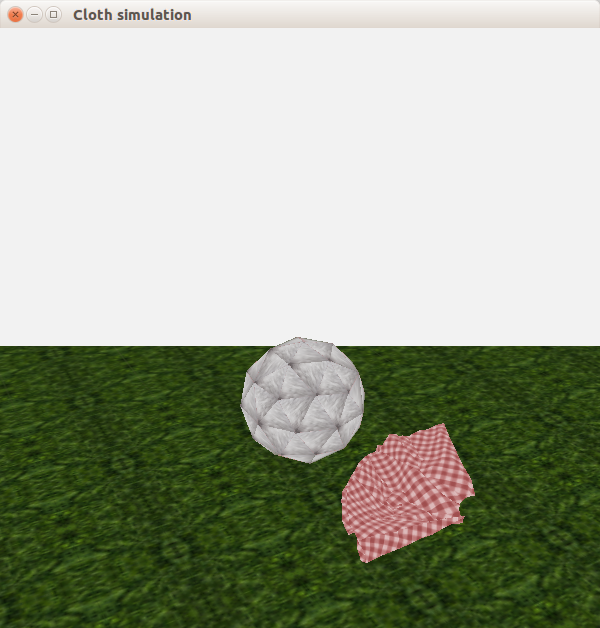
\includegraphics[width=\textwidth]{cloth_sim_skirt_on_floor}
		\subcaption{Finally the skirt falls down to the floor.}
		\label{fig:scene_floor}
	\end{subfigure}
	\caption{The cloth is initially placed above a sphere. It falls down onto the sphere and slips off to the floor.}
	\label{fig:scene}
\end{figure}
